% Provenance (never printed): cycle 4 SVT/physique, "La planete Terre,
% l'environnement": the atmosphere, its structure and its layers, pressure
% and altitude, the ozone layer; see sources/book1/PROVENANCE.md. Book 1,
% grade 8, chapter 1.
% Vocabulary guard: owns the layers of the atmosphere (troposphere,
% tropopause, stratosphere, mesosphere, thermosphere), the environmental
% lapse rate and the ozone layer. Air pressure and the barometer are the
% physics books' (recalled), the composition of air and ozone the molecule
% the chemistry books'; "convection cell" is g8.2's and is not used here;
% adiabatic cooling is Book 2's.
\chapter{वायुमंडल}\label{ch:g8:the-atmosphere}

किसी \omterm{def:g4:clouds-rain-snow:weather-station}{मौसम केंद्र} पर, तय समय से ठीक पहले, एक मौसम वैज्ञानिक हाइड्रोजन या हीलियम से भरा,
लगभग \qty{1.5}{m} चौड़ा एक गुब्बारा लेकर घास पर निकलती है। उसके नीचे, एक लंबी डोरी
पर, एक छोटा नारंगी पैराशूट और 60 से 80 ग्राम का एक उपकरण-डिब्बा लटका है: एक
\emph{रेडियोसोंड}। वह गुब्बारा छोड़ देती है। गुब्बारा हर मिनट लगभग \qty{300}{m}
चढ़ता है, और रेडियोसोंड हर सेकंड रेडियो से दाब, तापमान, आर्द्रता और अपनी स्थिति नीचे
भेजता है। ऊपर उठते हुए गुब्बारा फूलता जाता है, जब तक कि वह 6 से \qty{8}{m} चौड़ा
होकर फट नहीं जाता, अक्सर \qty{30}{km} से ज़्यादा ऊँचाई पर, छोड़े जाने के दो घंटे
बाद। हर दिन उन्हीं घंटों पर, यही दृश्य दुनिया भर के 800 से ज़्यादा केंद्रों पर
होता है।
% ledger: nws:radiosonde

\begin{omfigure}
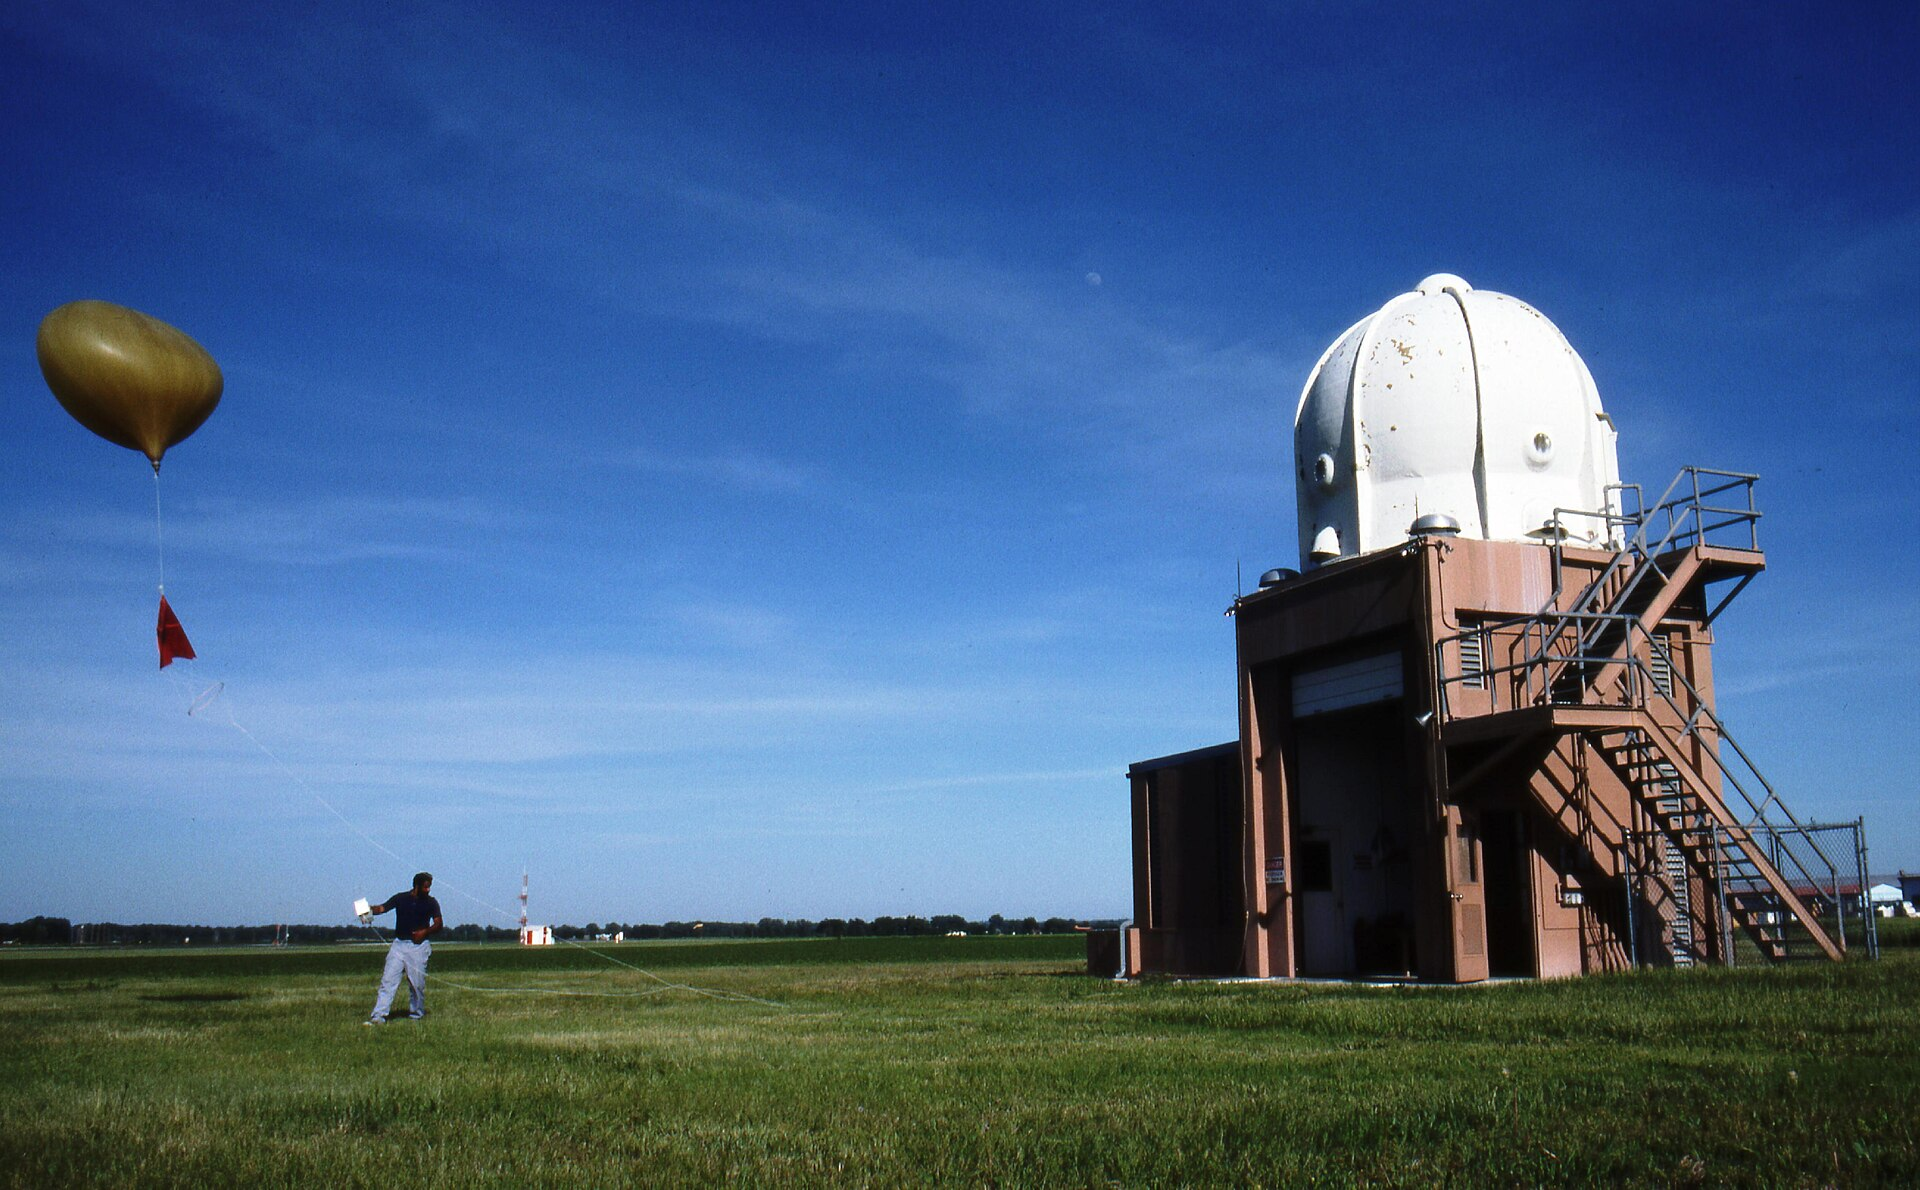
\includegraphics[width=0.78\linewidth]{images/book1/g8-radiosonde-launch.jpg}

{\small टोपेका, कैनसस (संयुक्त राज्य अमेरिका) में एक मौसमी गुब्बारा छोड़ा जा रहा है:
पैराशूट (लाल) और रेडियोसोंड गुब्बारे के नीचे लटके हैं। फ़ोटो: स्टीफ़न कोरफ़िडी,
NOAA/राष्ट्रीय \omterm{def:g1:watching-the-weather:weather}{मौसम} सेवा (सार्वजनिक डोमेन, विकिमीडिया कॉमन्स के
ज़रिए)।}
% ledger: commons:radiosonde-launch
\label{fig:g8:the-atmosphere:launch}
\end{omfigure}

ऊपर उठते हुए गुब्बारा क्यों फूलता है? ऊपर जाते हुए रेडियोसोंड क्या मापता है, और
तापमान बस गिरता ही क्यों नहीं जाता? हवा कहाँ ख़त्म होती
है?

\begin{recall}
\emph{वायुमंडल} पृथ्वी के चारों ओर हवा की परत है। हवा हर उस चीज़ पर दबाव डालती है
जिसे वह छूती है: यह \emph{वायुदाब} है, जिसे बैरोमीटर से मापा जाता है (भौतिकी की
किताबें)। \omterm{def:g1:watching-the-weather:weather}{मौसम} सेवाएँ इसे हेक्टोपास्कल (hPa) में देती हैं; \omterm{def:g4:world-physical-map:altitude}{समुद्र तल} पर यह लगभग
\qty{1013}{hPa} है। सूखी हवा लगभग 78~\% नाइट्रोजन और 21~\% ऑक्सीजन से बनी है,
साथ में थोड़ा आर्गन, कार्बन डाइऑक्साइड और दूसरी गैसें (रसायन विज्ञान की किताबें)।
\omterm{def:g4:clouds-rain-snow:cloud}{बादल} पानी की नन्ही बूँदों या बर्फ़ के क्रिस्टलों से बने होते हैं
(\cref{ch:g4:clouds-rain-snow})।
\end{recall}
% ledger: air:N2, air:O2, ussa76:sea-level

\section{एक पतला आवरण}

अंतरराष्ट्रीय अंतरिक्ष स्टेशन से देखने पर वायुमंडल पृथ्वी के किनारे पर एक पतली चमकती
रेखा है। ज़्यादातर हवा, और लगभग सारे \omterm{def:g4:clouds-rain-snow:cloud}{बादल}, उसके सबसे निचले कुछ किलोमीटरों में
हैं।
% ledger: commons:iss-sunset

\begin{omfigure}
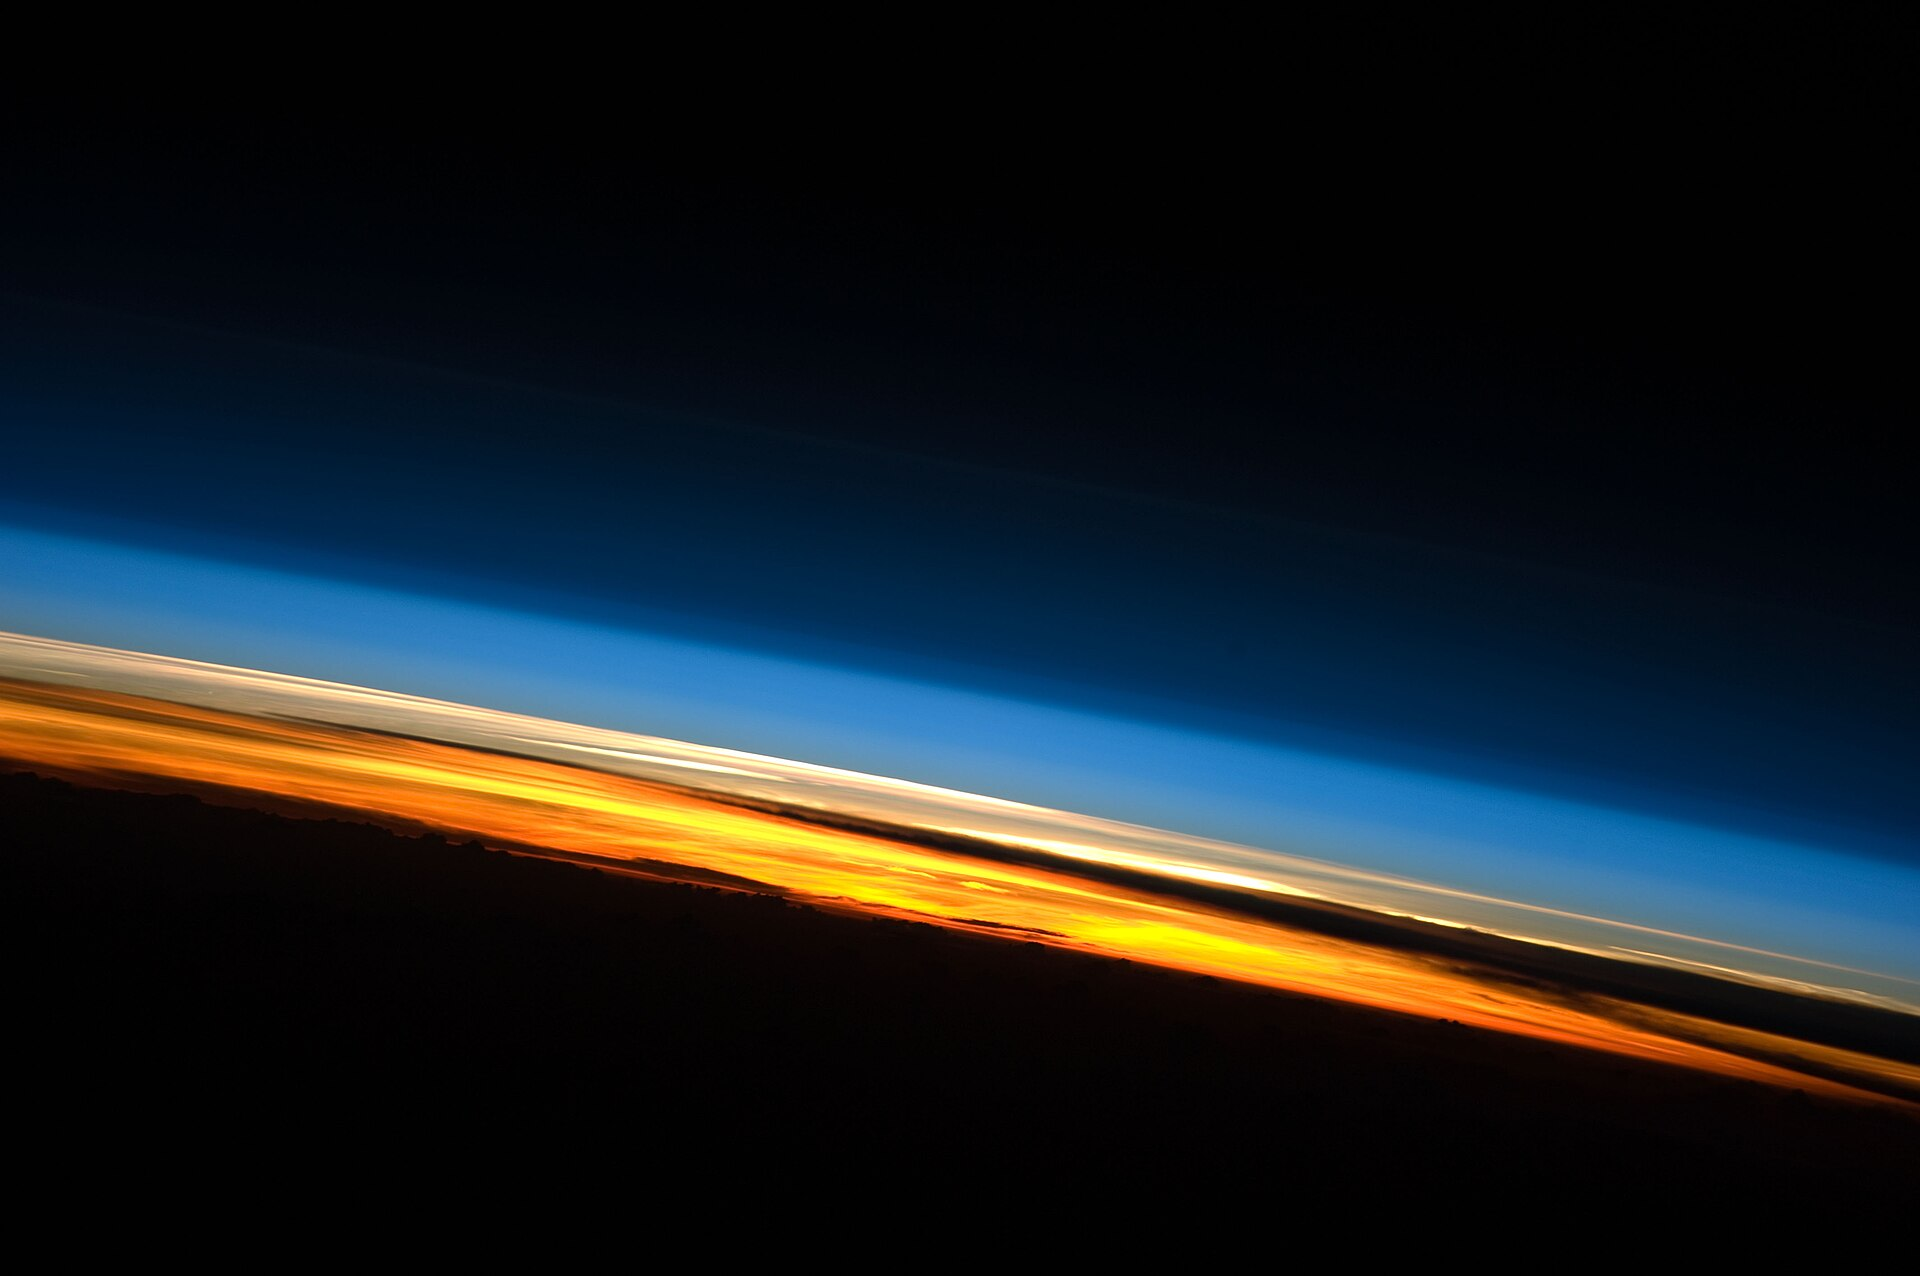
\includegraphics[width=0.78\linewidth]{images/book1/g8-iss-limb.jpg}

{\small सूर्यास्त के समय पृथ्वी का किनारा, 14~जून 2010 को हिंद \omterm{def:g2:water-on-earth:ocean}{महासागर} के ऊपर
अंतरराष्ट्रीय अंतरिक्ष स्टेशन से खींचा गया। नारंगी और पीली पट्टी वायुमंडल की सबसे
निचली परत है, अपने गहरे \omterm{def:g4:clouds-rain-snow:cloud}{बादलों} के साथ; उसके ऊपर हल्की और फिर नीली परतें आती हैं, जो
अंतरिक्ष के काले रंग में घुल जाती हैं। NASA फ़ोटो, ISS अभियान~23 (सार्वजनिक डोमेन,
विकिमीडिया कॉमन्स के ज़रिए)।}
% ledger: commons:iss-sunset
\label{fig:g8:the-atmosphere:limb}
\end{omfigure}

वायुमंडल का कोई तीखा ऊपरी सिरा नहीं है: ऊँचाई के साथ हवा पतली और पतली होती जाती है।
परंपरा से, अंतरिक्ष लगभग \qty{100}{km} पर शुरू होता है। पृथ्वी की त्रिज्या,
\qty{6371}{km}, की तुलना में यह बहुत कम है: $100 \div
6371 \approx 0.016$,
त्रिज्या के 2~\% से भी कम। \qty{30}{cm} चौड़े \omterm{def:g3:continents-and-oceans:globe}{ग्लोब} पर पूरा वायुमंडल लगभग
\qty{2}{mm} मोटी एक झिल्ली
होगा।
% ledger: ucar:layers, earth:Rmean

\begin{omfigure}
\begin{tikzpicture}[font=\footnotesize]
  % 1 cm = 100 km: the Earth's surface is a circle of radius 63.71 cm
  \def\R{63.71}
  \useasboundingbox (-6.9,-1.6) rectangle (6.9,1.0);
  \fill[blue!8] (0,-\R) ++(85:\R+1) arc (85:95:\R+1) -- ($(0,-\R)+(95:\R)$) arc (95:85:\R) -- cycle;
  \fill[omLithAlluv!70] (0,-\R) ++(85:\R) arc (85:95:\R) -- ++(0,-0.6) -- ($(0,-\R)+(85:\R)+(0,-0.6)$) -- cycle;
  \draw[black, line width=0.6pt] (0,-\R) ++(85:\R) arc (85:95:\R);
  \foreach \h/\c in {0.1102/omThm, 0.4938/omMeth, 0.86/omDef} \draw[\c, line width=0.5pt] (0,-\R) ++(85:\R+\h) arc (85:95:\R+\h);
  \draw[black!60, dashed] (0,-\R) ++(85:\R+1) arc (85:95:\R+1);
  \node[anchor=west, omThm] at (5.65,-0.14) {\qty{11}{km}};
  \node[anchor=west, omMeth] at (5.65,0.25) {\qty{49}{km}};
  \node[anchor=west, omDef] at (5.65,0.62) {\qty{86}{km}};
  \node[anchor=east, black!70] at (-5.65,0.75) {\qty{100}{km}};
  \node[anchor=north] at (0,-0.15) {पृथ्वी की सतह};
  \draw[|-|] (-5,-1.05) -- node[below] {\qty{1000}{km}} (5,-1.05);
\end{tikzpicture}

{\small पृथ्वी और उसके वायुमंडल की एक फाँक, पैमाने पर बनाई गई (\qty{1}{cm} बराबर
\qty{100}{km}), \qty{100}{km} तक, जो अंतरिक्ष का किनारा है (टूटी रेखा)। रंगीन
रेखाएँ उन परतों की सीमाएँ हैं जिनसे इस अध्याय में आगे मिलेंगे; सबसे निचली परत, जहाँ
सारा \omterm{def:g1:watching-the-weather:weather}{मौसम} होता है, मुश्किल से एक मिलीमीटर मोटी
है।}
% ledger: earth:Rmean, ucar:layers (limits: figdata/grade-8/standard_atmosphere.py main table)
\label{fig:g8:the-atmosphere:to-scale}
\end{omfigure}

\section{ऊँचाई के साथ दाब घटता है}

वायुमंडल के तल की हवा अपने ऊपर की सारी हवा का भार उठाती है। जितना ऊपर चढ़ो, ऊपर उतनी
कम हवा बचती है, और दाब उतना कम होता है। \omterm{def:g1:watching-the-weather:weather}{मौसम} वैज्ञानिकों और इंजीनियरों के उपयोग वाले
वायुमंडल के मानक मॉडल में, दाब \omterm{def:g4:world-physical-map:altitude}{समुद्र तल} पर \qty{1013}{hPa} है, लगभग
\qty{5.5}{km} पर उसका आधा, और लगभग \qty{10.3}{km} पर एक
चौथाई।
% ledger: ussa76:sea-level, ussa76:layers (figdata/grade-8/standard_atmosphere.py main table: half_km 5.48, quarter_km 10.29)

क्योंकि दाब ऊपर की हवा का भार मापता है, आधे दाब वाला स्तर वह ऊँचाई भी है जिसके नीचे
सारी हवा का आधा हिस्सा है: वायुमंडल का आधा हिस्सा उसके सबसे निचले \qty{5.5}{km} में
ठुँसा है। \qty{11}{km} के नीचे लगभग 78~\% हवा है, \qty{30}{km} के नीचे लगभग
99~\%।
% ledger: (computed: figdata/grade-8/standard_atmosphere.py, share_below_11km 77.7, share_below_30km 98.82)

\begin{omfigure}
\begin{minipage}[t]{0.49\linewidth}\centering
\begin{tikzpicture}
\begin{axis}[width=6.6cm, height=7.6cm, xmin=0, xmax=1100, ymin=0, ymax=30,
  xlabel={दाब (hPa)}, ylabel={ऊँचाई (km)},
  tick label style={font=\scriptsize}, label style={font=\small},
  xtick={0,250,500,750,1000}, ytick={0,5,10,15,20,25,30}]
  \addplot[dashed, black!60] table {figdata/out/grade-8-standard_atmosphere-guides.dat};
  \addplot[omDef, line width=1.1pt] table[x=p_hPa, y=z_km] {figdata/out/grade-8-standard_atmosphere-pressure.dat};
  \addplot[only marks, mark=*, mark size=1.8pt, omThm] table[x=p_hPa, y=z_km] {figdata/out/grade-8-standard_atmosphere-levels.dat};
  \node[anchor=south west, font=\scriptsize, text=black] at (axis cs:506.6,5.48) {आधा};
  \node[anchor=south west, font=\scriptsize, text=black] at (axis cs:253.3,10.29) {चौथाई};
\end{axis}
\end{tikzpicture}

{\small ऊँचाई के साथ दाब। लगभग \qty{5.5}{km} पर दाब \omterm{def:g4:world-physical-map:altitude}{समुद्र तल} के मान का आधा है,
लगभग \qty{10.3}{km} पर एक चौथाई।}
\end{minipage}\hfill
\begin{minipage}[t]{0.49\linewidth}\centering
\begin{tikzpicture}[font=\footnotesize]
  % at launch: 1.5 m; at burst: about 7 m (drawn 1 cm for 1.5 m)
  \draw[black!60] (0,0.9) -- (0,2.6);
  \shade[ball color=yellow!60!brown] (0,3.1) circle (0.5);
  \fill[red!75] (-0.25,1.75) .. controls (-0.2,2.05) and (0.2,2.05) .. (0.25,1.75) -- cycle;
  \fill[white, draw=black] (-0.15,0.55) rectangle (0.15,0.9);
  \node[anchor=north] at (0,0.45) {छोड़ते समय};
  \node[anchor=north] at (0,0.05) {\qty{1.5}{m} चौड़ा};
  \begin{scope}[xshift=3.1cm]
    \draw[black!60] (0,0.9) -- (0,2.6);
    \shade[ball color=yellow!40!white] (0,4.9) circle (2.3);
    \fill[red!75] (-0.25,1.75) .. controls (-0.2,2.05) and (0.2,2.05) .. (0.25,1.75) -- cycle;
    \fill[white, draw=black] (-0.15,0.55) rectangle (0.15,0.9);
    \node[anchor=north] at (0,0.45) {फटने से ठीक पहले};
    \node[anchor=north] at (0,0.05) {6 से \qty{8}{m} चौड़ा};
  \end{scope}
  \node[anchor=west, font=\scriptsize] at (0.3,1.9) {पैराशूट};
  \node[anchor=west, font=\scriptsize] at (0.3,0.72) {रेडियोसोंड};
\end{tikzpicture}

{\small चढ़ते हुए गुब्बारा फूलता है, क्योंकि उसके चारों ओर की हवा कम और कम दबाती है
(गुब्बारे और पैराशूट आपस में एक ही पैमाने पर, डोरी छोटी करके
दिखाई गई)।}
% ledger: nws:radiosonde
\end{minipage}
% ledger: ussa76:sea-level, ussa76:layers (figdata/grade-8/standard_atmosphere.py parts pressure, levels, guides)
\label{fig:g8:the-atmosphere:pressure}
\end{omfigure}

और ऊपर दाब गिरता ही रहता है, हर कुछ किलोमीटर पर फिर से लगभग आधा, इसलिए वह जल्दी ही
बहुत छोटा हो जाता है। उसे लिखने का सबसे अच्छा तरीक़ा दस की घातें हैं। \qty{30}{km}
पर दाब लगभग \qty{12}{hPa} है, \omterm{def:g4:world-physical-map:altitude}{समुद्र तल} के मान का मोटे तौर पर $10^{-2}$ (सौवाँ
हिस्सा); \qty{50}{km} पर लगभग \qty{0.8}{hPa}, मोटे तौर पर $10^{-3}$;
\qty{80}{km} पर लगभग \qty{0.01}{hPa}, \omterm{def:g4:world-physical-map:altitude}{समुद्र तल} के दाब का मोटे तौर पर $10^{-5}$।
% ledger: ussa76:layers (figdata/grade-8/standard_atmosphere.py main table: p_30km 11.97, p_50km 0.798, p_80km 0.0105 hPa)

\begin{omfigure}
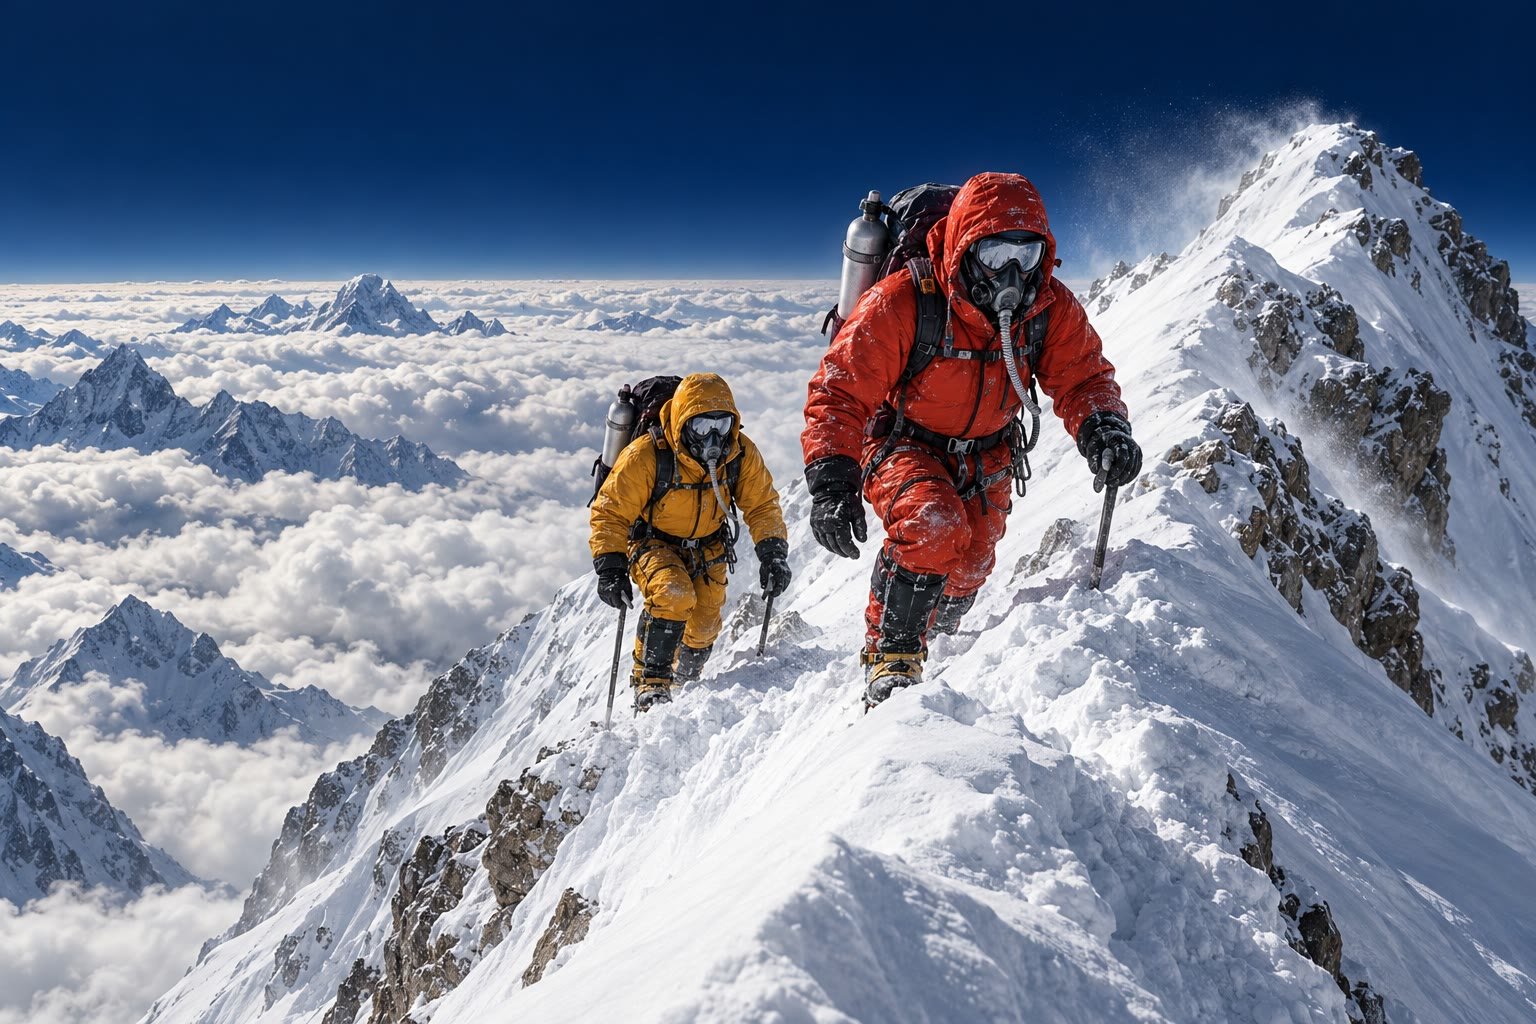
\includegraphics[width=0.5\linewidth]{images/book1/ai/g8-climbers.jpg}

{\small एक बहुत ऊँचे पहाड़ पर पर्वतारोही ऑक्सीजन की बोतलें ले जाते हैं। \qty{9}{km}
पर दाब \omterm{def:g4:world-physical-map:altitude}{समुद्र तल} के मान के एक तिहाई से भी कम है: हवा में अब भी 21~\% ऑक्सीजन है, पर
हर साँस उसे कहीं कम अंदर लेती है (एक सामान्य दृश्य का AI
चित्रण)।}
% ledger: air:O2 (figdata/grade-8/standard_atmosphere.py: pressure at 9 km 308 hPa, 30 % of sea level)
\label{fig:g8:the-atmosphere:climbers}
\end{omfigure}

\section{तापमान और परतें}

जिसने भी पहाड़ पर चढ़ाई की है, वह जानता है कि ऊँचाई के साथ हवा ठंडी होती जाती है।
रेडियोसोंड दिखाते हैं कि यह केवल वायुमंडल के सबसे निचले हिस्से में सच है। और ऊपर
तापमान गिरना बंद कर देता है, फिर बढ़ता है, फिर फिर से गिरता है, फिर एक बार और बढ़ता
है। ये बदलाव वायुमंडल को परतों में बाँटते
हैं।
% ledger: ucar:layers, ussa76:layers

\begin{omfigure}
\begin{tikzpicture}
\begin{axis}[width=10cm, height=9cm, xmin=-100, xmax=30, ymin=0, ymax=100,
  xlabel={तापमान ($^\circ$C)}, ylabel={ऊँचाई (km)},
  tick label style={font=\scriptsize}, label style={font=\small},
  xtick={-100,-80,-60,-40,-20,0,20}, ytick={0,10,20,30,40,50,60,70,80,90,100}, axis on top]
  \addplot[fill=omSea!55, draw=none] table {figdata/out/grade-8-standard_atmosphere-band-troposphere.dat};
  \addplot[fill=omMeth!12, draw=none] table {figdata/out/grade-8-standard_atmosphere-band-stratosphere.dat};
  \addplot[fill=omSea!35, draw=none] table {figdata/out/grade-8-standard_atmosphere-band-mesosphere.dat};
  \addplot[fill=omThm!10, draw=none] table {figdata/out/grade-8-standard_atmosphere-band-thermosphere.dat};
  \addplot[omThm, line width=1.2pt] table[x=T_C, y=z_km] {figdata/out/grade-8-standard_atmosphere-temp.dat};
  \node[anchor=west, font=\small\bfseries, text=black!75] at (axis cs:-97,5.51) {क्षोभमंडल};
  \node[anchor=west, font=\small\bfseries, text=black!75] at (axis cs:-97,30.2) {समतापमंडल};
  \node[anchor=west, font=\small\bfseries, text=black!75] at (axis cs:-97,67.69) {मध्यमंडल};
  \node[anchor=west, font=\small\bfseries, text=black!75] at (axis cs:-60,93) {तापमंडल};
  \draw[black!50, dashed] (axis cs:-100,11.02) -- (axis cs:30,11.02);
  \draw[black!50, dashed] (axis cs:-100,49.38) -- (axis cs:30,49.38);
  \draw[black!50, dashed] (axis cs:-100,86) -- (axis cs:30,86);
  \node[anchor=south east, font=\scriptsize] at (axis cs:17,11.02) {क्षोभसीमा};
  \node[anchor=south east, font=\scriptsize] at (axis cs:29,49.38) {समतापसीमा};
  \node[anchor=south east, font=\scriptsize] at (axis cs:29,86) {मध्यसीमा};
  \fill[omMeth!45] (axis cs:19,16) rectangle (axis cs:23,48);
  \node[anchor=east, font=\scriptsize, align=right] at (axis cs:18,30) {ओज़ोन\\परत};
\end{axis}
\end{tikzpicture}

{\small ऊँचाई के साथ हवा का तापमान, ज़मीन से \qty{100}{km} तक, मानक वायुमंडल में
(मध्य \omterm{def:g6:latitude-longitude:latitude}{अक्षांशों} का एक औसत)। चारों परतें रंगी गई हैं; हरी पट्टी \omterm{def:g8:the-atmosphere:ozone-layer}{ओज़ोन परत} की ऊँचाई
दिखाती है।}
% ledger: ussa76:sea-level, ussa76:layers, ussa76:above-86, ucar:ozone (figdata/grade-8/standard_atmosphere.py parts temp, layers, band-*)
\label{fig:g8:the-atmosphere:temperature}
\end{omfigure}

\begin{definition}[वायुमंडल की परतें]\label{def:g8:the-atmosphere:layers}
ज़मीन से ऊपर की ओर, ऊँचाई के साथ तापमान के बदलने के ढंग से वायुमंडल चार परतों में
बँटा है:
\begin{itemize}
  \item \emph{क्षोभमंडल}\index{क्षोभमंडल}, जहाँ ऊँचाई के साथ तापमान गिरता है और जहाँ
        लगभग सारा \omterm{def:g1:watching-the-weather:weather}{मौसम} होता है; उसका ऊपरी सिरा
        \emph{क्षोभसीमा}\index{क्षोभसीमा} है;
  \item \emph{समतापमंडल}\index{समतापमंडल}, जहाँ ऊँचाई के साथ तापमान बढ़ता है,
        लगभग \qty{50}{km} तक;
  \item \emph{मध्यमंडल}\index{मध्यमंडल}, जहाँ तापमान फिर से गिरता है, लगभग
        \qty{85}{km} तक;
  \item \emph{तापमंडल}\index{तापमंडल}, जहाँ बहुत पतली हवा ऊँचाई के साथ गरम और
        गरम होती जाती है।
\end{itemize}
\end{definition}
% ledger: ucar:layers, ussa76:layers

\omterm{def:g8:the-atmosphere:layers}{क्षोभमंडल} में वायुमंडल की लगभग 99~\% जलवाष्प है, इसलिए लगभग सारे \omterm{def:g4:clouds-rain-snow:cloud}{बादल}, वर्षा और \omterm{def:g4:clouds-rain-snow:precipitation}{हिम}
उसी में बनते हैं। उसकी हवा हर समय हिलती-मिलती रहती है। \omterm{def:g8:the-atmosphere:layers}{क्षोभमंडल} का ऊपरी सिरा हर
जगह एक ही ऊँचाई पर नहीं है: \omterm{def:g8:the-atmosphere:layers}{क्षोभसीमा} \omterm{def:g3:continents-and-oceans:equator}{भूमध्य रेखा} के ऊपर सबसे ऊँची है, जहाँ वह
\qty{20}{km} तक पहुँच सकती है, और \omterm{def:g3:continents-and-oceans:poles}{ध्रुवों} के ऊपर सबसे नीची, जहाँ जाड़े में वह
\qty{7}{km} तक उतर सकती है। वह जाड़े की तुलना में गर्मी में भी ऊँची होती है। मानक
वायुमंडल में, जो मध्य \omterm{def:g6:latitude-longitude:latitude}{अक्षांशों} का एक औसत है, वह \qty{11}{km} पर
है।
% ledger: ucar:layers, ucar:tropopause, ussa76:layers

\begin{definition}[पर्यावरणीय ह्रास दर]\label{def:g8:the-atmosphere:lapse-rate}
\emph{पर्यावरणीय ह्रास दर}\index{पर्यावरणीय ह्रास दर} वह दर है जिससे \omterm{def:g8:the-atmosphere:layers}{क्षोभमंडल} में
ऊँचाई के साथ हवा का तापमान गिरता है, डिग्री सेल्सियस प्रति किलोमीटर में। यह दिन-ब-दिन
और जगह-जगह बदलती है; मानक वायुमंडल \qty{6.5}{\degreeCelsius} प्रति किलोमीटर का
औसत लेता
है।
\end{definition}
% ledger: ussa76:layers

\begin{method}[तापमान का प्रोफ़ाइल पढ़ना]\label{met:g8:the-atmosphere:profile}
\begin{enumerate}
  \item खड़े अक्ष पर ऊँचाई ढूँढो और आड़े चलकर वक्र तक जाओ; उसके नीचे तापमान
        पढ़ो।
  \item जहाँ ऊपर जाते हुए वक्र बाईं ओर झुकता है, वहाँ ऊँचाई के साथ हवा ठंडी होती
        है; जहाँ वह दाईं ओर झुकता है, वहाँ ऊँचाई के साथ हवा गरम होती है; जहाँ वह
        खड़ा है, वहाँ तापमान नहीं बदलता।
  \item परतों के बीच की सीमाएँ वहाँ हैं जहाँ वक्र मुड़ता है।
\end{enumerate}
\end{method}

\begin{example}[क्रूज़िंग ऊँचाई पर एक यात्री विमान]\label{ex:g8:the-atmosphere:airliner}
एक यात्री विमान \qty{11}{km} पर, \omterm{def:g8:the-atmosphere:layers}{क्षोभसीमा} के पास, उड़ता है। प्रोफ़ाइल पर वहाँ तापमान
लगभग \qty{-56}{\degreeCelsius} है। ह्रास दर से: \omterm{def:g4:world-physical-map:altitude}{समुद्र तल} पर
\qty{15}{\degreeCelsius} से हवा $6.5 \times 11 = 71.5$ डिग्री ठंडी होती है, जिससे
$15 - 71.5 =
\qty{-56.5}{\degreeCelsius}$ मिलता है। दाब के वक्र पर दाब लगभग
\qty{227}{hPa} है, ज़मीन के दाब के एक चौथाई से भी कम: केबिन में दाब बनाए रखना
पड़ता है।
% ledger: ussa76:sea-level, ussa76:layers (figdata/grade-8/standard_atmosphere.py: T at 11 km -56.4 degC, p 227 hPa)
\end{example}

\omterm{def:g8:the-atmosphere:layers}{क्षोभसीमा} के ऊपर, \omterm{def:g8:the-atmosphere:layers}{समतापमंडल} में, यात्री विमानों की उड़ान ज़्यादा शांत होती है: वहाँ
ऊँचाई के साथ हवा गरम होती है, इसलिए वह नीचे से हिलती-मिलती नहीं। \omterm{def:g8:the-atmosphere:layers}{मध्यमंडल} में
ज़्यादातर उल्काएँ जल जाती हैं, और उसके ऊपरी सिरे पर, लगभग \qty{86}{km} पर, पूरे
वायुमंडल की सबसे ठंडी हवा है, लगभग \qty{-86}{\degreeCelsius}। \omterm{def:g8:the-atmosphere:layers}{तापमंडल} में सूर्य की
एक्स-किरणें और पराबैंगनी प्रकाश बहुत पतली हवा को सैकड़ों, कभी-कभी हज़ारों, डिग्री तक
गरम कर देते हैं; फिर भी वहाँ इतनी कम हवा है कि वह गरम महसूस नहीं होगी। बहुत-से
उपग्रह वहाँ पृथ्वी की परिक्रमा करते हैं।
% ledger: ucar:layers, ussa76:above-86

\section{ओज़ोन परत}

\omterm{def:g8:the-atmosphere:layers}{समतापमंडल} ऊँचाई के साथ इसलिए गरम होता है क्योंकि वह सूर्य के प्रकाश का कुछ हिस्सा
सोख लेता है। इसका ज़्यादातर काम करने वाली गैस ओज़ोन है, ऑक्सीजन का एक रूप (उसका
रसायन रसायन विज्ञान की किताबों में है)।

\begin{definition}[ओज़ोन परत]\label{def:g8:the-atmosphere:ozone-layer}
\emph{ओज़ोन परत}\index{ओज़ोन परत} \omterm{def:g8:the-atmosphere:layers}{समतापमंडल} का वह हिस्सा है, लगभग \qty{16}{km}
और \qty{48}{km} के बीच, जहाँ वायुमंडल की लगभग 90~\% ओज़ोन पाई जाती है। वह सूर्य
के ज़्यादातर हानिकारक पराबैंगनी प्रकाश को सोख लेती
है।
\end{definition}
% ledger: ucar:ozone

\omterm{def:g8:the-atmosphere:ozone-layer}{ओज़ोन परत} में भी ओज़ोन दुर्लभ है: दस लाख अणुओं में केवल 1 से 10। फिर भी ऑक्सीजन के
साथ मिलकर वह पृथ्वी तक पहुँचने वाले पराबैंगनी प्रकाश का 95~\% से 99.9~\% तक रोक
देती है, सबसे हानिकारक प्रकारों समेत। वह जो ऊर्जा सोखती है, ऊष्मा में बदल जाती है,
और इसीलिए \omterm{def:g8:the-atmosphere:layers}{समतापमंडल} में ऊपर जाते हुए तापमान बढ़ता है। \omterm{def:g8:the-atmosphere:ozone-layer}{ओज़ोन परत} के बिना, ज़मीन तक
पहुँचने वाला पराबैंगनी प्रकाश जीवों को नुक़सान
पहुँचाता।
% ledger: ucar:ozone

\begin{inthefield}[मौसमी गुब्बारों के पीछे-पीछे]
\omterm{def:g1:watching-the-weather:weather}{मौसम} सेवाएँ अपने रेडियोसोंडों के माप प्रकाशित करती हैं, अक्सर हर उड़ान के लिए ऊँचाई के
साथ तापमान के एक चार्ट के रूप में। किसी बड़े के साथ अपने सबसे पास के केंद्र की
00:00 या 12:00 UTC पर की गई मापें ढूँढो। वह ऊँचाई ढूँढो जहाँ तापमान गिरना बंद कर
देता है: वह उस दिन की \omterm{def:g8:the-atmosphere:layers}{क्षोभसीमा} है। जाड़े की किसी माप की तुलना गर्मी की किसी माप
से करो।
\end{inthefield}
% ledger: nws:radiosonde, ucar:tropopause

\section{अभ्यास}

\begin{exercise}[$\star$]\label{exo:g8:the-atmosphere:1}
हर परत को उसके वर्णन से मिलाओ: \omterm{def:g8:the-atmosphere:layers}{क्षोभमंडल}; \omterm{def:g8:the-atmosphere:layers}{समतापमंडल}; \omterm{def:g8:the-atmosphere:layers}{मध्यमंडल}; \omterm{def:g8:the-atmosphere:layers}{तापमंडल}। (क) वहाँ
ऊँचाई के साथ तापमान बढ़ता है और \omterm{def:g8:the-atmosphere:ozone-layer}{ओज़ोन परत} वहीं है। (ख) लगभग सारा \omterm{def:g1:watching-the-weather:weather}{मौसम} वहीं होता है।
(ग) वायुमंडल की सबसे ठंडी हवा उसके ऊपरी सिरे पर है। (घ) बहुत पतली हवा सैकड़ों डिग्री
तक गरम होती है; बहुत-से उपग्रह वहाँ परिक्रमा करते हैं।
\end{exercise}

\begin{exercise}[$\star$]\label{exo:g8:the-atmosphere:2}
मानक वायुमंडल के तापमान प्रोफ़ाइल का उपयोग करो। (क) \omterm{def:g4:world-physical-map:altitude}{समुद्र तल} पर तापमान क्या है?
(ख) \qty{11}{km} पर? (ग) \qty{50}{km} पर? (घ) \qty{86}{km} पर? (ङ) किन
ऊँचाइयों के बीच तापमान नहीं
बदलता?
\end{exercise}

\begin{exercise}[$\star$]\label{exo:g8:the-atmosphere:3}
सही या ग़लत? ग़लत वाक्यों को सुधारो। (क) ऊँचाई के साथ हवा का तापमान हमेशा गिरता है।
(ख) सारी हवा का आधा हिस्सा लगभग \qty{5.5}{km} के नीचे है। (ग) \omterm{def:g8:the-atmosphere:ozone-layer}{ओज़ोन परत}
\omterm{def:g8:the-atmosphere:layers}{क्षोभमंडल} में है। (घ) \omterm{def:g8:the-atmosphere:layers}{क्षोभसीमा} \omterm{def:g3:continents-and-oceans:poles}{ध्रुवों} की तुलना में \omterm{def:g3:continents-and-oceans:equator}{भूमध्य रेखा} के ऊपर ज़्यादा ऊँची
है।
\end{exercise}

\begin{exercise}[$\star$]\label{exo:g8:the-atmosphere:4}
इनमें से हर एक किस परत में है? (क) वर्षा वाला एक \omterm{def:g4:clouds-rain-snow:cloud}{बादल}। (ख) \qty{12}{km} पर एक
यात्री विमान। (ग) फटने से ठीक पहले, \qty{32}{km} पर, एक मौसमी गुब्बारा।
(घ) \qty{75}{km} पर जलती एक उल्का।
\end{exercise}

\begin{exercise}[$\star\star$]\label{exo:g8:the-atmosphere:5}
गर्मी के एक दिन \omterm{def:g4:world-physical-map:altitude}{समुद्र तल} पर \qty{20}{\degreeCelsius} है। मान लो हवा
\qty{6.5}{\degreeCelsius} प्रति किलोमीटर ठंडी होती है। (क) \qty{2}{km} पर तापमान
क्या है? (ख) \qty{3}{km} पर? (ग) लगभग किस ऊँचाई पर हवा \qty{0}{\degreeCelsius} तक
पहुँचती है? एक दशमलव स्थान तक पूर्णांकित करो।
\end{exercise}

\begin{exercise}[$\star\star$]\label{exo:g8:the-atmosphere:6}
एक \omterm{def:g1:landscapes-around-us:landform}{पहाड़ी} कुटिया \qty{3000}{m} पर है। एक पैदल यात्री \qty{500}{m} पर बसे एक गाँव
से चलता है, जहाँ \qty{18}{\degreeCelsius} है। \qty{6.5}{\degreeCelsius} प्रति
किलोमीटर की ह्रास दर का उपयोग करके: (क) पैदल यात्री कितने किलोमीटर चढ़ता है? (ख) हवा
कितने डिग्री ठंडी होती है? (ग) पैदल यात्री कुटिया पर किस तापमान की उम्मीद कर
सकता है?
\end{exercise}

\begin{exercise}[$\star\star$]\label{exo:g8:the-atmosphere:7}
मान लो हर \qty{5.5}{km} पर दाब आधा हो जाता है, \omterm{def:g4:world-physical-map:altitude}{समुद्र तल} पर \qty{1000}{hPa} से शुरू
करके। (क) \qty{5.5}{km} पर दाब क्या है? \qty{11}{km} पर? \qty{16.5}{km} पर?
(ख) मानक वायुमंडल इन तीन ऊँचाइयों पर लगभग \qty{506}{hPa}, \qty{227}{hPa} और
\qty{96}{hPa} देता है (\omterm{def:g4:world-physical-map:altitude}{समुद्र तल} पर \qty{1013}{hPa} के लिए)। क्या आधे होने का नियम
ज़मीन के पास अच्छा है? और ऊपर?
\end{exercise}

\begin{exercise}[$\star\star$]\label{exo:g8:the-atmosphere:8}
\omterm{def:g4:world-physical-map:altitude}{समुद्र तल} पर दाब लगभग \qty{1000}{hPa} है, यानी $10^3$~hPa। (क) \qty{30}{km} पर
वह लगभग \qty{10}{hPa} है। इसे दस की घात के रूप में लिखो, और बताओ कि यह \omterm{def:g4:world-physical-map:altitude}{समुद्र तल} से
कितने गुना छोटा है। (ख) \qty{80}{km} पर वह लगभग \qty{0.01}{hPa} है। इसे दस की
घात के रूप में लिखो। (ग) यह \omterm{def:g4:world-physical-map:altitude}{समुद्र तल} से कितने गुना छोटा
है?
\end{exercise}

\begin{exercise}[$\star\star$]\label{exo:g8:the-atmosphere:9}
एक मौसमी गुब्बारा छोड़ते समय \qty{1.5}{m} चौड़ा है और फटते समय \qty{6}{m} चौड़ा।
(क) फटते समय वह कितने गुना चौड़ा है? (ख) समझाओ कि ऊपर उठते हुए वह क्यों फूलता है।
(ग) \omterm{def:g1:watching-the-weather:weather}{मौसम} सेवाएँ उसके नीचे पैराशूट क्यों लटकाती
हैं?
\end{exercise}

\begin{exercise}[$\star\star$]\label{exo:g8:the-atmosphere:10}
\omterm{def:g8:the-atmosphere:layers}{क्षोभसीमा} \omterm{def:g3:continents-and-oceans:equator}{भूमध्य रेखा} के ऊपर \qty{20}{km} तक पहुँच सकती है और जाड़े में \omterm{def:g3:continents-and-oceans:poles}{ध्रुवों} के
ऊपर \qty{7}{km} तक उतर सकती है। (क) इस स्थिति में \omterm{def:g3:continents-and-oceans:equator}{भूमध्य रेखा} के ऊपर \omterm{def:g8:the-atmosphere:layers}{क्षोभमंडल}
कितने गुना मोटा है? एक दशमलव स्थान तक पूर्णांकित करो। (ख) मानक प्रोफ़ाइल पर
\omterm{def:g8:the-atmosphere:layers}{क्षोभसीमा} \qty{11}{km} पर है। मानक वायुमंडल \omterm{def:g3:continents-and-oceans:equator}{भूमध्य रेखा} के ज़्यादा पास है या \omterm{def:g3:continents-and-oceans:poles}{ध्रुवों}
के? (ग) एक पायलट \qty{10}{km} की एक-सी ऊँचाई पर किसी ध्रुवीय क्षेत्र से \omterm{def:g3:continents-and-oceans:equator}{भूमध्य रेखा}
तक उड़ता है। शुरुआत में (जाड़े में) विमान \omterm{def:g8:the-atmosphere:layers}{क्षोभमंडल} में है या \omterm{def:g8:the-atmosphere:layers}{समतापमंडल} में? अंत
में?
\end{exercise}

\begin{exercise}[$\star\star\star$]\label{exo:g8:the-atmosphere:11}
किसी ऊँचाई के नीचे की हवा का हिस्सा $1 - p \div
p_0$ है, जहाँ $p$ उस ऊँचाई पर दाब
है और $p_0 =
\qty{1013}{hPa}$ \omterm{def:g4:world-physical-map:altitude}{समुद्र तल} पर दाब। (क) \qty{5.5}{km} पर
$p
\approx \qty{506}{hPa}$: हवा का कितना हिस्सा नीचे है? (ख) \qty{11}{km} पर
$p \approx \qty{227}{hPa}$। (ग) \qty{30}{km} पर $p \approx
\qty{12}{hPa}$। जवाब
प्रतिशत में, पूर्ण संख्याओं तक, दो। (घ) \qty{30}{km} के ऊपर हवा का कितना हिस्सा है?
\end{exercise}

\begin{exercise}[$\star\star\star$]\label{exo:g8:the-atmosphere:12}
स्कूल का एक \omterm{def:g3:continents-and-oceans:globe}{ग्लोब} \qty{30}{cm} चौड़ा है, इसलिए उसकी त्रिज्या, \qty{15}{cm}, पृथ्वी
की त्रिज्या, \qty{6371}{km}, को दर्शाती है। (क) \omterm{def:g3:continents-and-oceans:globe}{ग्लोब} का \qty{1}{cm} कितने
किलोमीटर दर्शाता है? निकटतम किलोमीटर तक पूर्णांकित करो। (ख) \qty{100}{km} तक का
वायुमंडल इस \omterm{def:g3:continents-and-oceans:globe}{ग्लोब} पर कितने मिलीमीटर मोटा होगा? (ग) और \qty{11}{km} मोटा
\omterm{def:g8:the-atmosphere:layers}{क्षोभमंडल}? (घ) काग़ज़ की एक शीट लगभग \qty{0.1}{mm} मोटी है। \omterm{def:g3:continents-and-oceans:globe}{ग्लोब} का \omterm{def:g8:the-atmosphere:layers}{क्षोभमंडल}
कितनी शीटों से बनेगा?
\end{exercise}

\section{समस्या: एक मौसमी गुब्बारे के पीछे-पीछे}

\begin{problem}[{सप्ताहांत समस्या --- एक मौसमी गुब्बारा वायुमंडल में चढ़ता है;
उसके तापमान परतों को दिखाते हैं, और उसके दाब दिखाते हैं कि समुद्र तल के दाब का एक
चौथाई कहाँ बचता है}]
\label{pb:g8:the-atmosphere:1}
% ledger: nws:radiosonde; the table is the standard atmosphere, figdata/grade-8/standard_atmosphere.py part sonde
\omterm{def:g4:world-physical-map:altitude}{समुद्र तल} पर बसे एक केंद्र से एक रेडियोसोंड छोड़ा जाता है। उसका गुब्बारा लगभग
\qty{300}{m} प्रति मिनट उठता है। तालिका वह दाब और तापमान देती है जो वह मापता है (मानक
वायुमंडल के मान, पूर्णांकित)।

\begin{center}\small
\begin{tabular}{|l|*{8}{c|}}
\hline
ऊँचाई (km) & 0 & 2 & 4 & 6 & 8 & 10 & 12 & 14 \\
\hline
दाब (hPa) & 1013 & 795 & 617 & 472 & 357 & 265 & 194 & 142 \\
\hline
तापमान ($^\circ$C) & 15 & 2 & $-11$ & $-24$ & $-37$ & $-50$ & $-56$ & $-56$ \\
\hline
\hline
ऊँचाई (km) & 16 & 18 & 20 & 22 & 24 & 26 & 28 & 30 \\
\hline
दाब (hPa) & 104 & 76 & 55 & 40 & 30 & 22 & 16 & 12 \\
\hline
तापमान ($^\circ$C) & $-56$ & $-56$ & $-56$ & $-55$ & $-53$ & $-51$ & $-49$ & $-47$ \\
\hline
\end{tabular}
\end{center}

\noindent\textbf{भाग I --- चढ़ाई।}\par\nopagebreak
\begin{enumerate}[beginpenalty=10000]
  \item 10 मिनट में गुब्बारा कितने मीटर चढ़ता है?
  \item \qty{6}{km} तक पहुँचने में उसे कितना समय लगता है? और \qty{30}{km} तक?
  \item गुब्बारा \qty{30}{km} पर फटता है। उड़ान कितनी देर चली, घंटों और मिनटों
        में?
  \item उस परत का नाम बताओ जिसमें गुब्बारा \qty{8}{km} पर है, और उस परत का जिसमें
        वह फटते समय है।
\end{enumerate}

\noindent\textbf{भाग II --- तापमान।}\par\nopagebreak
\begin{enumerate}[resume, beginpenalty=10000]
  \item ज़मीन और \qty{10}{km} के बीच तापमान कितने डिग्री गिरता है?
  \item चढ़ाई के इस हिस्से में ह्रास दर कितने डिग्री प्रति किलोमीटर
        है?
  \item किन ऊँचाइयों के बीच तापमान एक-सा रहता है? \omterm{def:g8:the-atmosphere:layers}{क्षोभसीमा} कहाँ
        है?
  \item \qty{20}{km} के ऊपर तापमान के साथ क्या होता है? कौन-सी गैस इसे समझाती
        है?
\end{enumerate}

\noindent\textbf{भाग III --- दाब।}\par\nopagebreak
\begin{enumerate}[resume, beginpenalty=10000]
  \item \omterm{def:g4:world-physical-map:altitude}{समुद्र तल} के दाब का आधा कितना है? यह किन ऊँचाइयों के बीच पहुँचा जाता
        है?
  \item \omterm{def:g4:world-physical-map:altitude}{समुद्र तल} के दाब का एक चौथाई कितना है? निकटतम हेक्टोपास्कल तक पूर्णांकित
        करो।
  \item तालिका की किन दो ऊँचाइयों के बीच यह चौथाई पहुँचा जाता है?
  \item \qty{10}{km} और \qty{12}{km} के बीच दाब \qty{71}{hPa} गिरता है। मान लो
        यह बराबर-बराबर गिरता है, तो लगभग किस ऊँचाई पर दाब \omterm{def:g4:world-physical-map:altitude}{समुद्र तल} के मान का एक
        चौथाई है? एक दशमलव स्थान तक पूर्णांकित
        करो।
\end{enumerate}
\end{problem}
